\documentclass[12pt,a4paper]{article}
\usepackage[ddmmyyyy]{datetime}
\renewcommand{\dateseparator}{.}
\usepackage[T1]{fontenc}
\usepackage[utf8]{inputenc}
\usepackage{graphicx} % Grafikleri eklemek için gerekli paket
\graphicspath{{images/}} % Grafik yolu belirleme
\renewcommand{\figurename}{Şekil}
\usepackage{geometry}
%\usepackage{natbib}
\usepackage{pdflscape} %Landscape format	
\usepackage[export]{adjustbox}
\renewcommand{\refname}{Kaynakça}
\usepackage{subcaption}
\usepackage{caption}
\usepackage[utf8]{inputenc}

\title{\bf\fontsize{12pt}{14pt}\selectfont KÜTAHYA SAĞLIK BİLİMLERİ ÜNİVERSİTESİ \\ MÜHENDİSLİK VE DOĞA BİLİMLERİ FAKÜLTESİ}

\begin{document}
	\maketitle
	\thispagestyle{empty}
	\begin{center}
		
\includegraphics{images/ksbu.png}
	\end{center}
	\begin{center}
		\vspace{1cm} % Vertical space of 1cm
	\end{center}
	\begin{center}
		\title{\bf\fontsize{12pt}{14pt}\selectfont YAPAY ZEKA DERSİ FİNAL RAPORU }
	\end{center}
	\begin{center}
		\title{\bf\fontsize{12pt}{14pt}\selectfont İNSANLARIN KÖPEKLERDEN KORKMASINI ENGELLEME}
	\end{center}
	\begin{center}
		\vspace{1cm} % Vertical space of 1cm
	\end{center}
	\begin{center}
		
		%\title{\bf\fontsize{12pt}{14pt}\selectfont Hande Öz\hspace{1.5cm}2118121038}	
		\author{\bf\fontsize{12pt}{14pt}Hande Öz\hspace{1.5cm}2118121038}
		
		\begin{center}
			\vspace{1cm} % Vertical space of 1cm
		\end{center}
		\begin{center}
			\vspace{1cm} % Vertical space of 1cm
		\end{center}
	\end{center}
	
	\section{Giriş} 
		Bu projede, hayvanlara karşı korku duygusu besleyen insanların korkularını azaltmak veya ortadan kaldırmak için yapay zeka algoritmalarından A* algoritması ve Unreal Engine oyun motoru kullanılacaktır. A* algoritması, hayvan ile insan arasındaki mesafeyi gerçek zamanlı olarak belirlemek için kullanılırken, Unreal Engine ise bu mesafeye göre sanal bir ortam oluşturmak ve kullanıcıyı bu ortamda hayvanlarla etkileşime sokmak için kullanılması amaçlanmaktadır.
		
		
		\section{Literatür Taraması}
		\begin{enumerate}
			\item[a)] Projemize yakın olarak yapılan çalışmalar vardır 
			Bu makalede, sinofobi (köpekten korkma) tedavisinde sanal gerçeklik maruziyetine dayalı terapinin etkinliği araştırılmıştır. Özellikle, işitsel-görsel ortamların duygu ve varlık üretme etkinliği incelenmiştir.
			Sinofobi, hem görsel hem de işitsel bileşenleri olan bir fobi türüdür.Makalede, sinofobi tedavisinde sanal gerçeklik tabanlı maruz bırakma terapisinin etkisini değerlendirmek için çeşitli sanal ortamlar kullanılmıştır. Bu ortamlar, çeşitli anksiyojenik durumların simülasyonlarını içermektedir ve farklı düzeylerde görsel ve işitsel uyarıcılar içermektedir.\newline
			
			İlk Ortam: Bu sanal ortamda, bir koridor bulunmaktadır. Eğitim ortamında ağaçlar, bir ev, masalar, ve banklardan oluşan bir bahçe de bulunmaktadır.\newline
			
			İkinci Ortam: Bu ortam, büyük ve karanlık bir hangarda yer alan bir iç mekanı simüle etmektedir. Bu ortamda, farklı endüstriyel makine parçaları aktif ve gürültülü bir şekilde gösterilmektedir. Ayrıca, bu ortamlarda birkaç köpek aşamalı olarak gösterilmiştir.\newline
	
	
			 Bu projede tereoskopik Görüntüleme,3D Ses,Kafa Takip Sistemi,Kablosuz Joystick gibi teknolojiler kullanılmıştır.
			 \pagenumbering{gobble} %Sayfa numaralandırması kalkıyor
			\pagenumbering{arabic} %Sayfa numaralandırmasını bu sayadan başlat
			\setcounter{page}{1}.
			
			
			Projede, sanal gerçeklik (VR) teknolojisini kullanarak sinofobi (köpeklerden korkma) tedavisi amaçlamaktadır. Kullanıcılar, bu sanal ortamda rahatlama ve sakinleşmeyi teşvik eden işitsel ve görsel uyaranlara maruz kalmaktadır. \newline
			Bu çalışmada gerekli koşullar sağlandığında köpek korkusunun önüne geçilebileceği görülmüştür\cite{MarinaTaffou}.\newline
		
			\item[b)]  
			Bu makale bir çocuğun köpek korkusunu yenmesine yönelik bir çalışmadır.
			Bu çalışma hayvanat bahçesinde geçiyor orada sorumlu olan adam bu makalede çocuğun küçükken bir köpeğin üzerine atladığını  bu yüzden köpeklerden korktuğunu ve köpeklerin dişlerinden korktuğunu  öğreniyor.
			
			Hayvanat bahçesinde, sorumlu bir kişi çocuğun korkusunu yenmesi için ona eşlik etmiş ve 8 seansta, melez bir köpek olan Zoti ile çocuğun arasında bir bağ kurmayı başarmıştır.
			İlk seansta daha önce sırtında bir tümör olan kısa süre önce ameliyatla alınan sağlıklı bir  köpek olan zotinin hastalığını cocuk öğrenmiş ve üzülmüş köpekte çocuğun üzüldüğünü anlamış gibi iç çekmiş insan empati testlerinde başarılı olan insanlar hayvanların duygusal seslerini çözmede de ölçülebilir derecede daha iyidirler sonraki seanslarda sorumlu kişi  köpeğe uzaktan ödül maması verdirtmiş sonrasında çocuk yakınlaşarak ödül maması vermiş yeterli miktarda zaman çocuk ile köpeği aynı ortamda bulundurmuş çocuğu köpeğe adım adım yaklaştırmıştır.
			
			
			doğru köpek ve yaklaşımla köpek korkusu üstesinden gelinebilir işin püf noktası başlangıçta doğru tür köpekle eşleşmek ve hastayı zorlamamak,doğru miktarda zaman ayırmak ve onlara korkularının normal oldugunu ancak bunun sadece bir korku olduğunu ve onunla yüz yüze ilgilenerek kesinlikle yenebileceklerini göstermektedir\cite{ahsan2023deep}. \newline \newline

	\end{enumerate}
		\section{Metodoloji} 
		
		\begin{itemize}
			\item Unreal Engine:Unreal Engine, Epic Games tarafından geliştirilen bir oyun motorudur. Unreal Engine, oyun geliştiricilerine oyun dünyalarını oluşturmak, 3D modelleme, fizik ve animasyon gibi çeşitli özelliklerle oyunların geliştirilmesine olanak tanır. Ayrıca, sanal gerçeklik (VR) kullanılabilir. 
			\item Python:Python, kullanımı kolay,yüksek seviyeli bir bir programlama dilidir.Web geliştirme, veri analizi, yapay zeka, oyun geliştirme ve daha birçok alanda kullanılır. 
			\item Blueprint:Blueprint, Unreal Engine'in görsel programlama sistemi olarak bilinir. Geliştiricilere kod yazmadan oyun ve uygulamalar oluşturmak için bir araç sağlar. Bir kullanıcı arayüzü kullanarak, nesneler arasında ilişkiler kurabilir, etkileşimler belirleyebilir.
		     	\item Aktör:Aktörler,statik olmayan nesneleri temsil etmek için de kullanılabilir, bir oyuncu karakteri, bir ışık kaynağı gibi.
		     	\item Static mesh(Statik Kafes):Bir nesnenin sabit ve değişmez bir şekilde tanımlandığı bir 3B model türüdür. Bu tür nesneler, genellikle oyun dünyasında sabit nesneleri temsil etmek için kullanılır ,duvar,taş gibi
		     	\begin{center}
		     			\begin{figure}[!htbp]
		     			\includegraphics[width=0.7\textwidth,center]{images/agac.png}
		     			\caption{projenin sahnesi}
		     			\label{fig:ornek}
		     		\end{figure}
		     	\end{center}
		     	 \begin{flushleft}
		     		Sahnede  yukarıdaki  bahçe kullanabilir.
		     	\end{flushleft}
		     	\item Static mesh foliage:Static mesh nesnesinin miktarını artırmak veya azaltmak için kullanılan bir araçtır(yeşillik,ağaç).
		     		\begin{center}
		     		\begin{figure}[htbp]
		     			\centering
		     			\begin{minipage}{0.45\textwidth}
		     				\centering
		     				\includegraphics[
		     				width=7cm,
		     				height=7cm,
		     				keepaspectratio,]{agac.png}
		     				\caption{fırça yoğunluğu(brush size) fazla}
		     			\end{minipage}
		     			\hfill
		     			\begin{minipage}{0.45\textwidth}
		     				\centering
		     				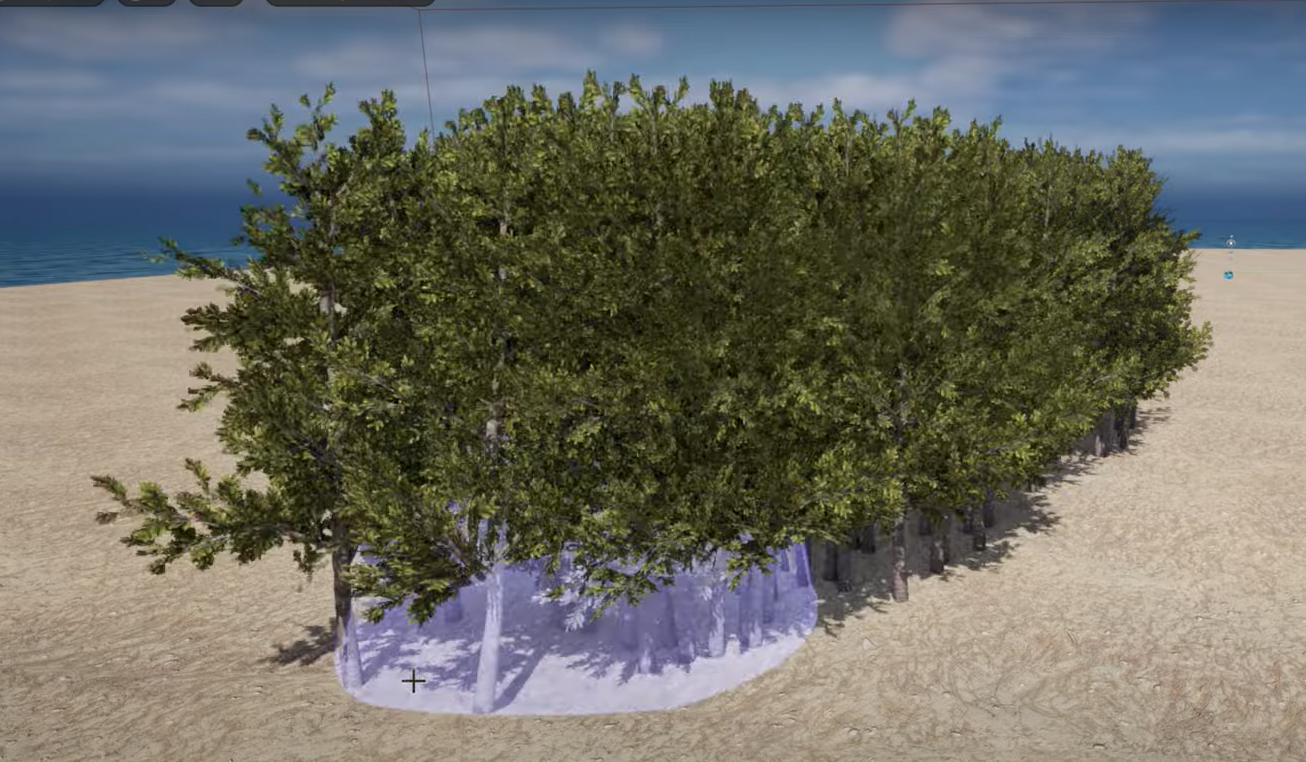
\includegraphics[
		     				width=7cm,
		     				height=7cm,
		     				keepaspectratio,]{sıkagac.png}
		     				\caption{fırça yoğunluğu(brush size) az}
		     			\end{minipage}
		     		\end{figure}
		     	\end{center}
		     	\item Skeletal mesh(İskelet Kafes):Bir nesnenin hareketli veya değişken bir şekilde tanımlandığı bir 3B model türüdür. Bu tür nesneler, genellikle karakterlerin veya canavarların animasyonlu hareketlerini temsil etmek için kullanılır.
			\item Asset: Bir oyun motorunda veya dijital içerik üretim aracında kullanılan her türlü grafik, model, ses, animasyon, metin dosyası gibi içerikler asset olarak adlandırılır. Bu, oyun geliştiricilerin projelerinde kullanabilecekleri kaynak dosyalarını ifade eder.
			\item Animasyon yansıtma: bir karakterin bir tarafındaki animasyonu diğer tarafa kopyalayarak aynı animasyonu farklı durumlarda yeniden kullanmanızı sağlar. Aynı zamanda Unreal Engine içindeki yansıtma, ikinci bir kopyayı yönetmeye gerek kalmadan yansıtılmış animasyonlar oluşturmanın bir yolunu sağlar. 
			\item İnput mapping context:VR gözlüğü kullanırken Input Mapping Context'leri, kullanıcının oyun içindeki farklı bağlamlarda farklı eylemleri gerçekleştirmesine izin vermek için oldukça yararlı olabilir. Örneğin, kullanıcının VR'da hareket etmesi, nesneleri alması veya bırakması gibi farklı eylemler için farklı kontroller sağlanabilir.\newline		
			\begin{center}
				\begin{figure}[htbp]
					\centering				
					\begin{subfigure}[t]{0.7\textwidth}
					
						\label{fig:ornek1}
						
						\centering
						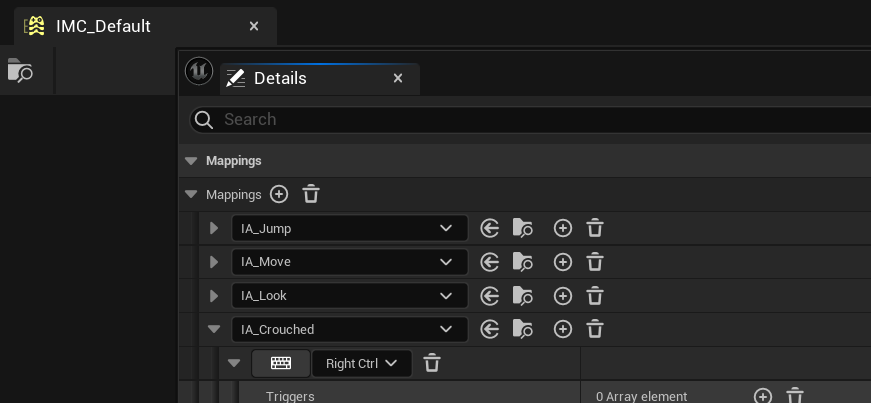
\includegraphics[width=\textwidth]{images/inputmapping.png}
							\caption{}
					\end{subfigure}
					\begin{subfigure}[t]{0.7\textwidth}
					
						\label{fig:ornek2}
						
						\centering
						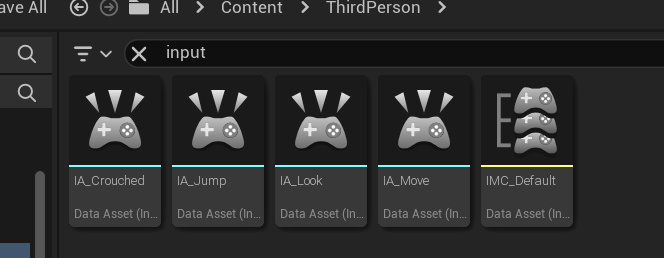
\includegraphics[width=\textwidth]{images/inputac.png}
							\caption{}
					\end{subfigure}
					\caption{a)Input örneği   b)Input mapping context örneği}
					\label{fig:ornekler}
				\end{figure}
			\end{center}
		
			
		
			\item Animation blueprint:Yazdığımız blueprint kodları ile  animasyonun senkronize bir şekilde çalışması,karmaşık animasyon davranışlarının oluşturulması ve kontrolü için kullanılan görsel komut dosyalarıdır.			
		\begin{center}
			\begin{figure}[!htbp]
				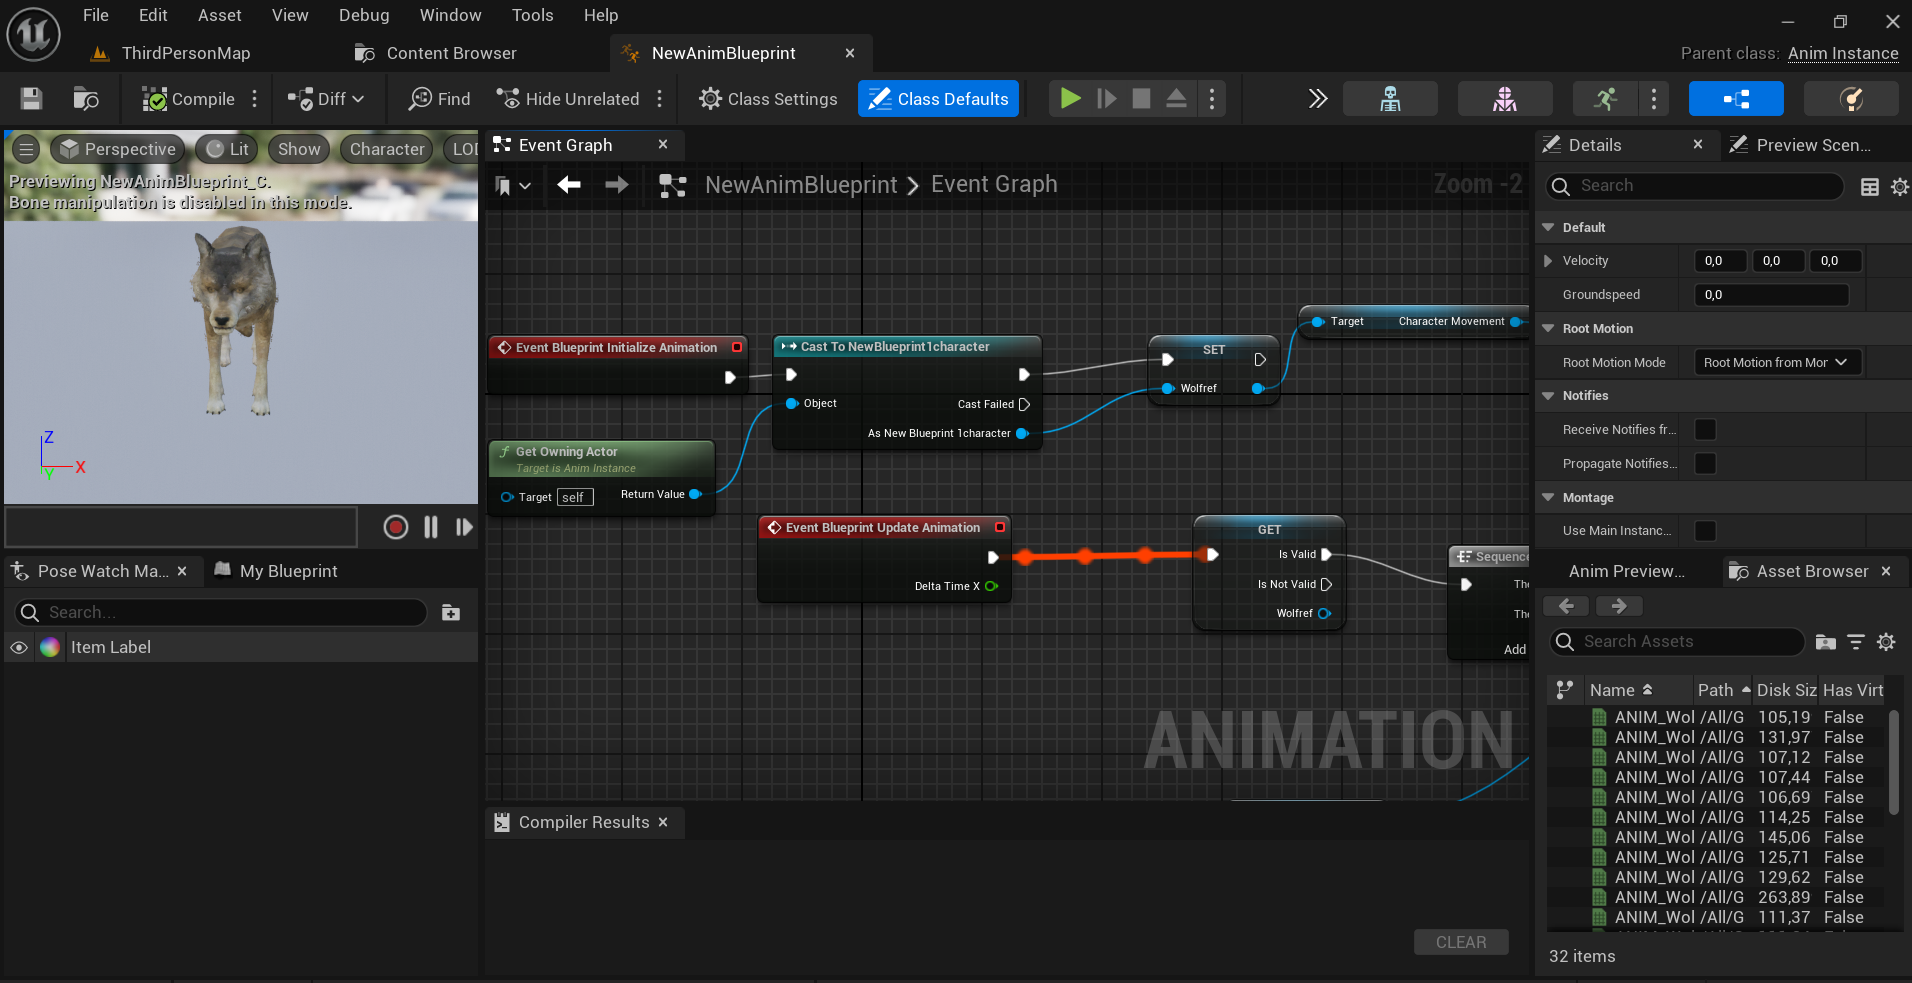
\includegraphics[width=0.7\textwidth,center]{images/anblue.png}
				\caption{Animasyon bluprint  örneği}
				\label{fig:ornek}
			\end{figure}
	 	\end{center}
		
			\item Blend space:birden fazla animasyon veya şekil arasında geçiş yapmayı sağlayan bir tekniktir.Animasyonların yumuşak ve doğal görünmesini sağlar çünkü animasyonların ani geçişler yerine doğal bir şekilde birbirine karışmasını sağlar.
			\begin{center}
				\begin{figure}[!htbp]
				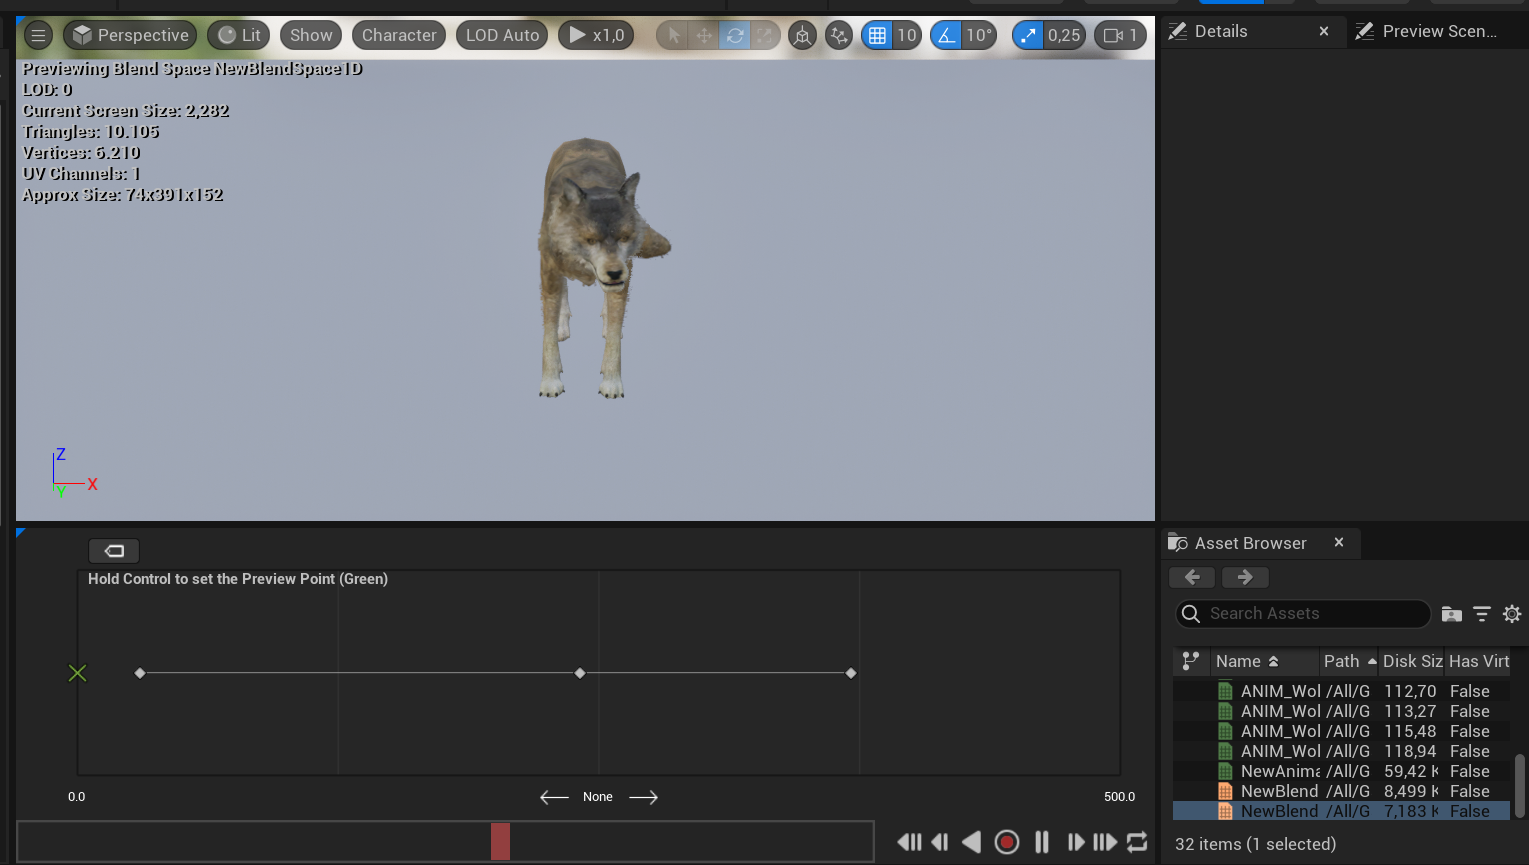
\includegraphics[width=0.7\textwidth,center]{images/blend.png}
				\caption{Blend space  örneği}
				\label{fig:ornek}
			\end{figure}
			\end{center}
		
			\item Finite State machine:Belirli animasyonları tanımlamak ve ne zaman oynatılabilceğini belirtmek için Animasyon Blueprint'lerde oluşturabileceğiniz modüler sistemlerdir.Başlıca olarak, bu tür bir sistem, karakterlerinizin hareket durumlarıyla animasyonları ilişkilendirmek için kullanılır.
	\begin{center}
		\begin{figure}[htbp]
		\centering
		
		\begin{subfigure}[t]{0.7\textwidth}
		
			\label{fig:ornek1}
			\centering
			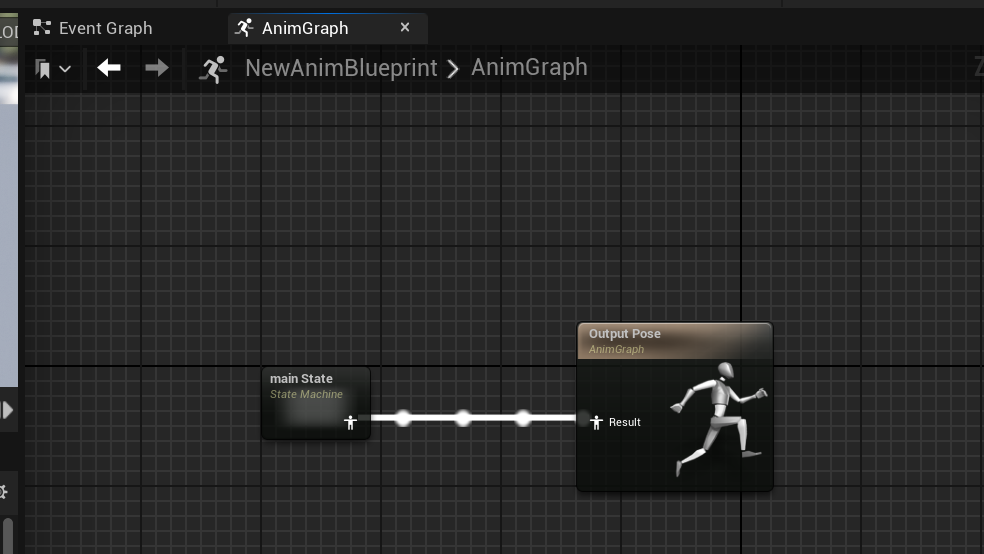
\includegraphics[width=\textwidth]{images/machine.png}
				\caption{}
		\end{subfigure}
		\begin{subfigure}[t]{0.7\textwidth}
		
			\label{fig:ornek2}
			\centering
			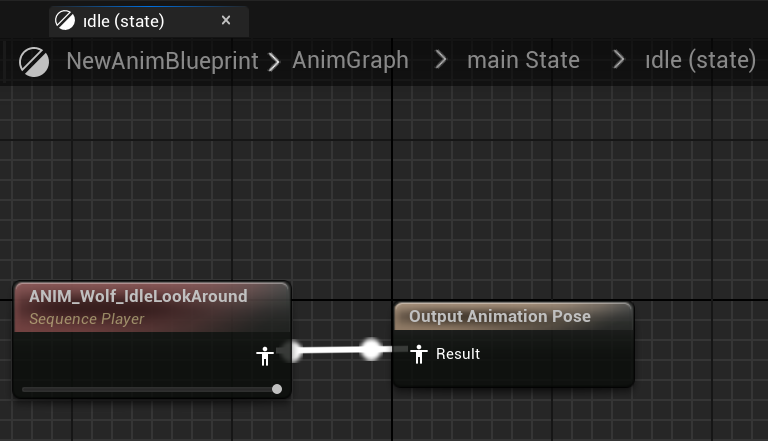
\includegraphics[width=\textwidth]{images/ıdle.png}
				\caption{}
		\end{subfigure}
		\begin{subfigure}[t]{0.7\textwidth}
			
			\label{fig:ornek2}
			\centering
			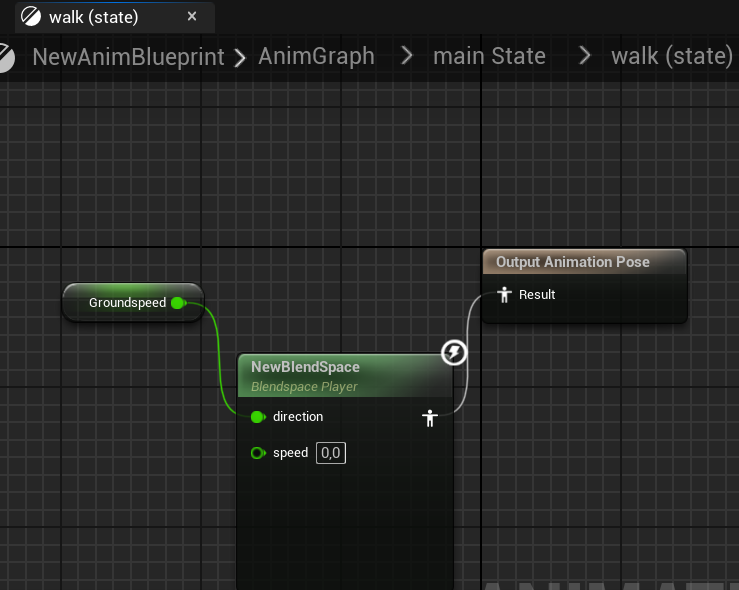
\includegraphics[width=\textwidth]{images/walk.png}
			\caption{}
		\end{subfigure}
		\caption{a)Durum makinesi örneği b)Durma örneği c)Yürüme örneği }
		\label{fig:ornekler}
    	\end{figure}
	\end{center}
					
			\item Karakter hareket bileşeni(character movement component): insan benzeri karakterler için yürüme, düşme, yüzme ve uçma da dahil olmak üzere ortak hareket modlarıyla kapsüllenmiş bir hareket sistemi sağlayan bir Aktör Bileşenidir. Karakter hareket bileşeni aynı zamanda sağlam ağ oyunu entegrasyonuna sahiptir. Varsayılan hareket modları varsayılarak yapılmıştır ve geliştiricilere özel ağ iletişimli hareketler oluşturmalarına yardımcı olacak bir çerçeve sunar.\newline\newline
			\begin{center}
				\begin{figure}[!htbp]
				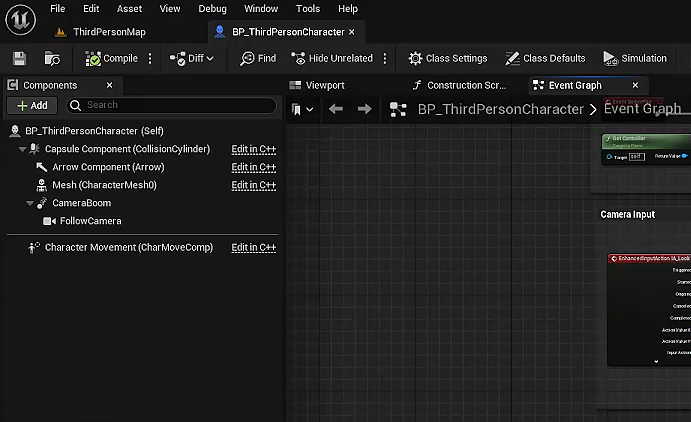
\includegraphics[width=0.7\textwidth,center]{images/kar.png}
				\caption{Karakter  örneği}
				\label{fig:ornek}
			   \end{figure}
			\end{center}
			
		    \item Inverse Kinematics (ters kinematik) :Bir nesnenin veya bir karakterin belirli bir hedefe doğru hareketini hesaplamak için kullanılan bir matematiksel yöntemdir.karakterlerin ellerini, ayaklarını veya diğer vücut parçalarını gerçekçi bir şekilde hareket ettirebilme imkanı sunar.
		    \begin{center}
		    	\begin{figure}[!htbp]
		    	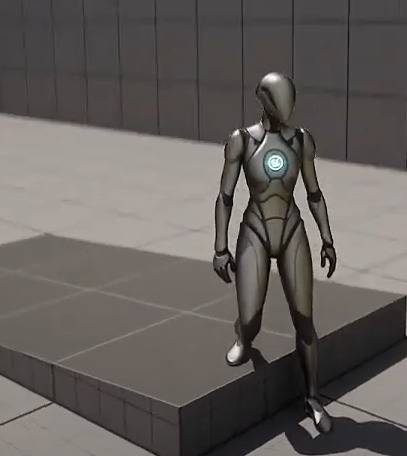
\includegraphics[width=0.7\textwidth,center]{images/ık.png}\newline
		    	\caption{IK  örneği}
		    	\label{fig:ornek}
		    \end{figure}
		    \end{center}
		 \begin{center}
		 	\begin{figure}[!htbp]
		 	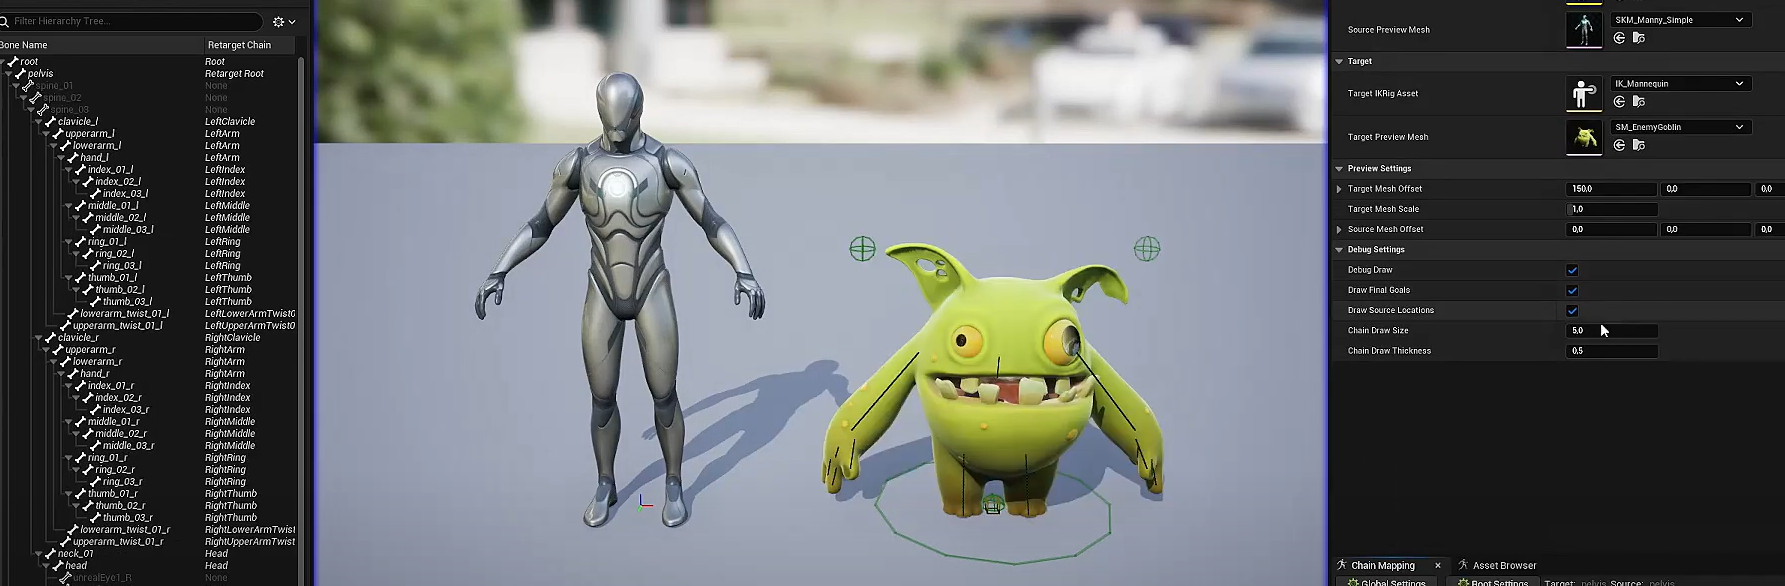
\includegraphics[width=0.7\textwidth,center]{images/esle.png}\cite{youtube}
		 	\caption{Kemik eşleştirme  örneği}
		 	\label{fig:ornek}
		 \end{figure}
		 \end{center}
		 	 	\item Hareket eşleştirme(Motion matching): Unreal Engine'de karakter animasyonlarının daha gerçekçi ve doğal görünmesini sağlayan bir tekniktir. Bu teknik, karakterin hareketlerini gerçek zamanlı olarak analiz ederek, en uygun animasyonun seçilmesini ve oynatılmasını sağlar.
		 	 
		 	 Motion matching, karakterin çeşitli durumlara uygun animasyonların geçişlerini daha doğal hale getirir ve oyuncunun kontrolünü arttırır. Bu sayede karakterin hareketleri daha gerçekçi ve akıcı bir şekilde gözükür.
		 	 
		 	 \item Savaş sistemi(Combat system):
		 	 Unreal Engine'de combat system, oyuncuların düşmanlarla etkileşimde bulunurken kullanabilecekleri çeşitli mekanikleri ve özellikleri içeren bir sistemdir. Bu sistem genellikle saldırı, savunma, hareket ve diğer benzeri ögeleri içerir.
		 	  Combat system, genellikle animasyonlar, vuruş ve savunma mekanikleri, düşman yapay zekası, sağlık ve hasar sistemleri gibi çeşitli bileşenleri içerir. Bu bileşenlerin bir araya gelmesiyle oyuncuların düşmanlarla etkileşime geçebileceği gerçekçi ve heyecan verici bir savaş deneyimi oluşturulur.
		 	 Unreal Engine'de combat system oluşturmak için Blueprint veya C++ gibi programlama dilleri kullanılabilir. Ayrıca Unreal Engine Marketplace'te hazır combat system paketleri bulunabilir.
		 	 \item A* algoritması:A* arama algoritması, sezgisel bir çizge dolaşma ve en kısa yol bulma algoritmasıdır\cite{astar}.
		 	 \item Varsayılan sahne kökü(Default Scene Root): Unreal Engine'de aktörlerin hiyerarşik yapısını ve dönüşümlerini yönetmek için temel bir bileşendir. Her aktörde otomatik olarak oluşturulur ve yeni sahne bileşenleri eklemek ve aktörünüzün konumunu ve rotasyonunu kontrol etmek için kullanılabilir. 
		 	 \item  Tetikleme için başlama olayı(OnActorBeginOverlap)->Başka bir aktör bu aktörle örtüşmeye başladığında çağrılır, örneğin bir oyuncunun tetikleyiciye girmesi. Nesnelerin engelleyici çarpışmaya sahip olduğu olaylar için, örneğin bir oyuncunun duvara çarpması \cite{overlap}.
		 	 \item Tetik kutusu (trigger box):Belirli bir alanda bir şeyin gerçekleşmesini tetikleyen bir bileşendir. Örneğin, bir karakter belirli bir alana girdiğinde bir olayın gerçekleşmesini sağlayabilir.
		 	 \item  Tetik olayı (trigger Event):gerçekleşen bir olayı işlemek için kullanılan bir fonksiyondur. Örneğin, bir trigger box'a giren bir karakter için bir event oluşturarak bu karakterin belirli bir animasyonu oynatmasını sağlayabilirsiniz.
		 	
		 	 \item Statik ağ üzerinde çarpışma (Collisions on Static Meshes):Çarpışma, dünyanızdaki nesnelerin kesişmesini engelleyen şeydir. Çarpışma olmadan oyuncu ağın içinden yürüyebilir\cite{collision}.
		 	 
		 	 \begin{center}
		 	 	\begin{figure}[htbp!]
		 	 		\centering				
		 	 		\begin{subfigure}[t]{0.7\textwidth}
		 	 			
		 	 			\label{fig:ornek1}
		 	 			
		 	 			\centering
		 	 			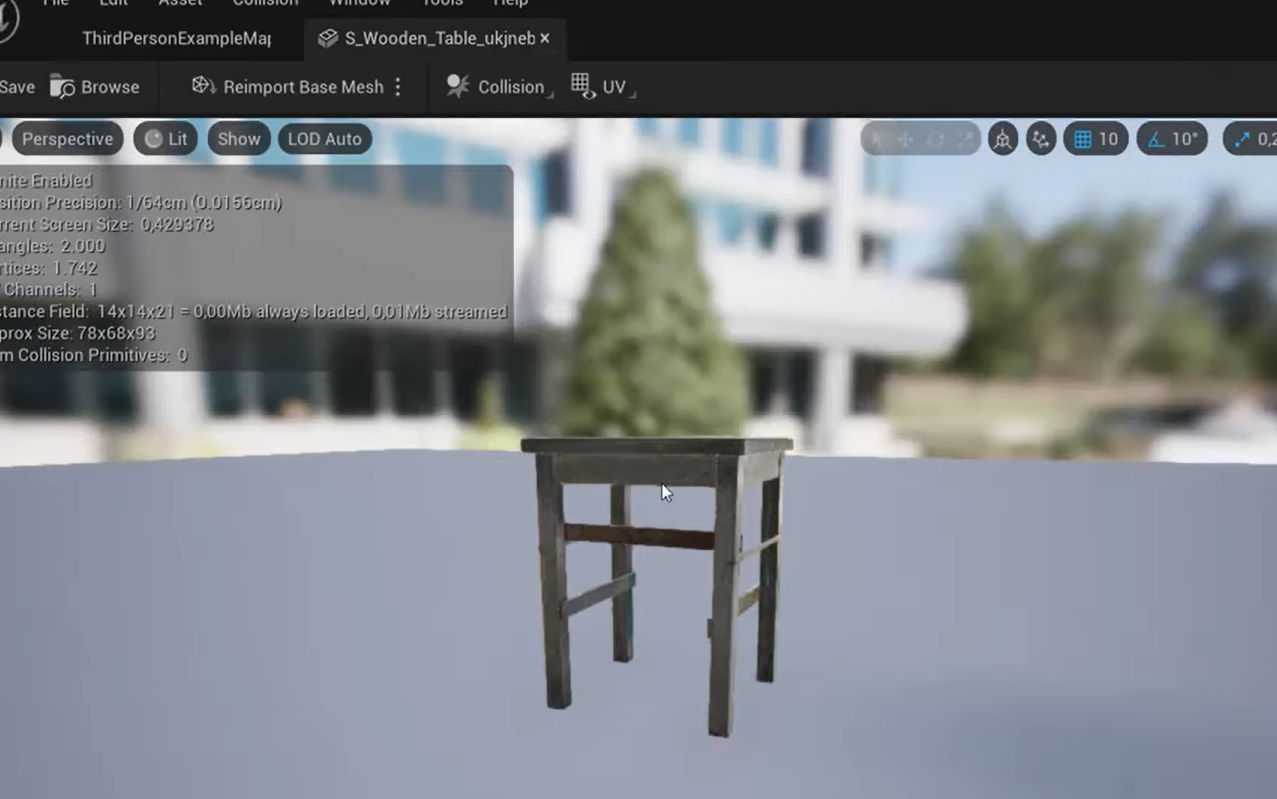
\includegraphics[width=\textwidth]{images/collision.png}
		 	 			\caption{}
		 	 		\end{subfigure}
		 	 		\begin{subfigure}[t]{0.7\textwidth}
		 	 			
		 	 			\label{fig:ornek2}
		 	 			
		 	 			\centering
		 	 			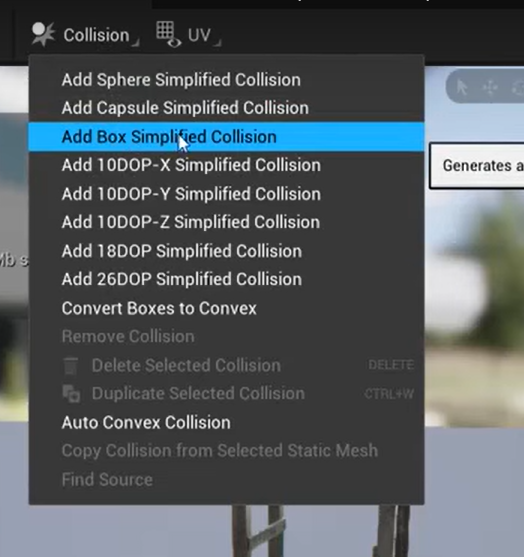
\includegraphics[width=\textwidth]{images/collision2.png}
		 	 			\caption{}
		 	 		\end{subfigure}
		 	 		\caption{a)Çarpışma Penceresi   b)Nesneye göre çarpışma türü seçimi}
		 	 		\label{fig:ornekler}
		 	 	\end{figure}
		 	 \end{center}
		
		 	 \item widget blueprint:Widget BP (Blueprint) görsel arayüz elementleri oluşturmak ve yönetmek için kullanılan bir araçtır. Oyunlarda menüler,Dikkat Göstergesi (HUD(Heads-Up Display)) elementleri, diyalog kutuları gibi arayüz öğelerini oluşturmak için kullanılır.
		 	 \item Eklentiler(plugins) :Eklentiler, geliştiricilerin Editör içinde proje bazında kolayca etkinleştirip devre dışı bırakabileceği kod ve veri koleksiyonlarıdır. Eklentiler, çalışma zamanı oyun işlevselliği ekleyebilir, yerleşik Motor özelliklerini değiştirebilir (veya yenilerini ekleyebilir), yeni dosya türleri oluşturabilir ve Düzenleyicinin yeteneklerini yeni menüler, araç çubuğu komutları ve alt modlarla genişletebilir.a star eklemek için kullanılabilir.
		 	 Projemizde Landmass plugin kullanılmıştır, genellikle oyun dünyasında büyük ve detaylı araziler oluşturmak için kullanılır. Bu eklenti sayesinde kullanıcılar, kolayca dağlar, vadiler, nehirler ve diğer doğal öğeleri oluşturabilir ve düzenleyebilirler.
		 	 
		 	 Landmass plugin, Unreal Engine'in Landscape sistemi ile entegre çalışır ve daha hızlı ve verimli bir arazi oluşturma süreci sunar. Ayrıca, kullanıcılar için çeşitli arazi oluşturma araçları ve özellikler sağlar.
		 	  \begin{center}
		 	 	\begin{figure}[!htbp]
		 	 		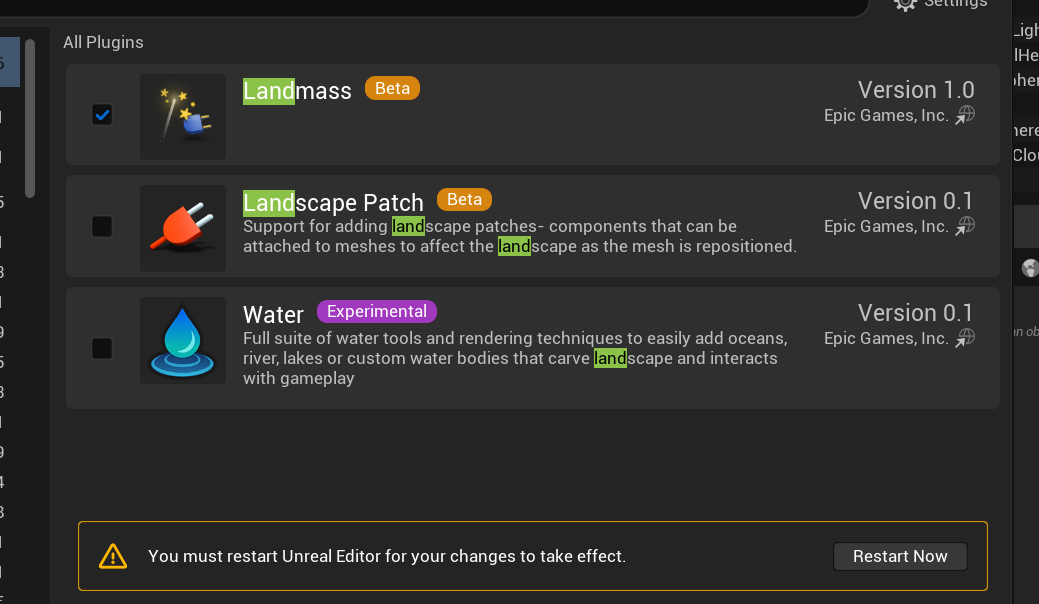
\includegraphics[width=0.7\textwidth,center]{images/landmass.png}\newline
		 	 		\caption{Eklenti  örneği}
		 	 		\label{fig:ornek}
		 	 	\end{figure}
		 	\end{center}
		 	 	
		 	   Hem rasterizasyon hem de ray tracing, bilgisayar grafiklerinde kullanılan, ekranınızdaki veya Render düğmesine bastığınızda sabit diskinizde oluşturulan resmin renklerini belirlemek için kullanılan renderleme yöntemleridir. Rasterizasyon, bir sahnedeki nesneleri arkadan öne doğru çizerek çalışır, 3D nesneleri dönüş matrisleri aracılığıyla 2D düzleme eşler. Her pikselin rengini, modele (ağa) saklanan bilgilere (renk, doku, normal) ve sahnedeki ışıkla birleştirilerek belirler. Genellikle ray tracingden çok daha hızlıdır, ancak gerçek yansımalar, saydamlık ve çevresel oklüzyon gibi yansıyan ışığa dayalı etkileri simüle edemez.
		 	 \item Işın izleme(Ray tracing):kameranın bakış noktasından bir ışın fırlatarak çalışır ve ışığa ulaşana kadar sahnede nesneler arasında yansıyarak yolunu izlerken renkleri toplar ve bırakır. Işık ışınlarının fiziksel davranışını taklit ettiği için, yumuşak, detaylı gölgeler, ambiyanstan kesilme ve doğru kırılma ve yansımalar gibi rasterleştirme yönteminden çok daha yüksek kaliteli, daha fotogerçekçi sonuçlar sunar. Ancak, tüm bu avantajlar geleneksel olarak bir maliyetle gelir: hız.
		 	 
		 	 Unreal Engine 5'in gelişmiş ışın izleme teknolojisini kullanarak gerçekçi görseller oluşturmasını sağlayan bir grafik özelliğidir. Bu teknoloji sayesinde ışık, gölge ve yansımalar daha gerçekçi bir şekilde simüle edilebilir.
		 		 
		 	
		 	 
		 	 	\item Malzeme örneği(Material Instance): Unreal Engine gibi oyun motorlarında kullanılan bir özelliktir. Bu özellik sayesinde bir malzeme (material) örneğini oluşturabilir ve bu örneği farklı nesnelerde veya sahnelerde kullanabilirsiniz. Bu sayede aynı malzeme örneğini farklı nesnelerde kullanarak bellek kullanımını azaltabilir ve işlemci performansını artırabilir.
		 	\item Bileşeni yakala(Grab component):Unreal Engine'de bir nesneyi tutma ve taşıma işlemlerini gerçekleştirmek için kullanılan bir bileşendir. Bu bileşen genellikle bir karakter veya oyuncu karakteri tarafından kullanılır ve bir nesneyi tutup taşımak için kullanılır.
		 	Grab component, genellikle bir fizik bileşeni ile birlikte kullanılır ve nesnelerin fiziksel özelliklerini etkileyerek gerçekçi bir taşıma deneyimi sağlar. Bu bileşen aynı zamanda nesnenin tutulma ve bırakılma olaylarını da yönetir.
		 	\item Yumurtlayan aktör (Spawning actor):Bir Aktörün yeni bir örneğini yaratma süreci,belirtilen sınıfın yeni bir örneğini oluşturur ve yeni oluşturulan Aktöre bir işaretçi döndürür\cite{spawn}.
		 	\item Olay dağıtıcısı(Event dispactcher ):Bir veya daha fazla olayı bir Olay Dağıtıcısına bağlayarak,Olay Dağıtıcısı çağrıldığında tüm bu olayların tetiklenmesini sağlayabiliriz\cite{eventdis}.
	    \item Gezinme ağı sınırları hacmi (Nav Mesh Bounds Volume):AI karakterlerinin hareket etmesini sağlayan bir bileşendir. Bu bileşen, AI karakterlerinin hareket alanını belirlemek için kullanılır \cite{aıalan}.
	     \end{itemize}
	     
	     	
	\newpage
		\section{Gantt Chart ve İş Akış Planı \newline} 
	\begin{figure}[!htbp] 		
		\centering
		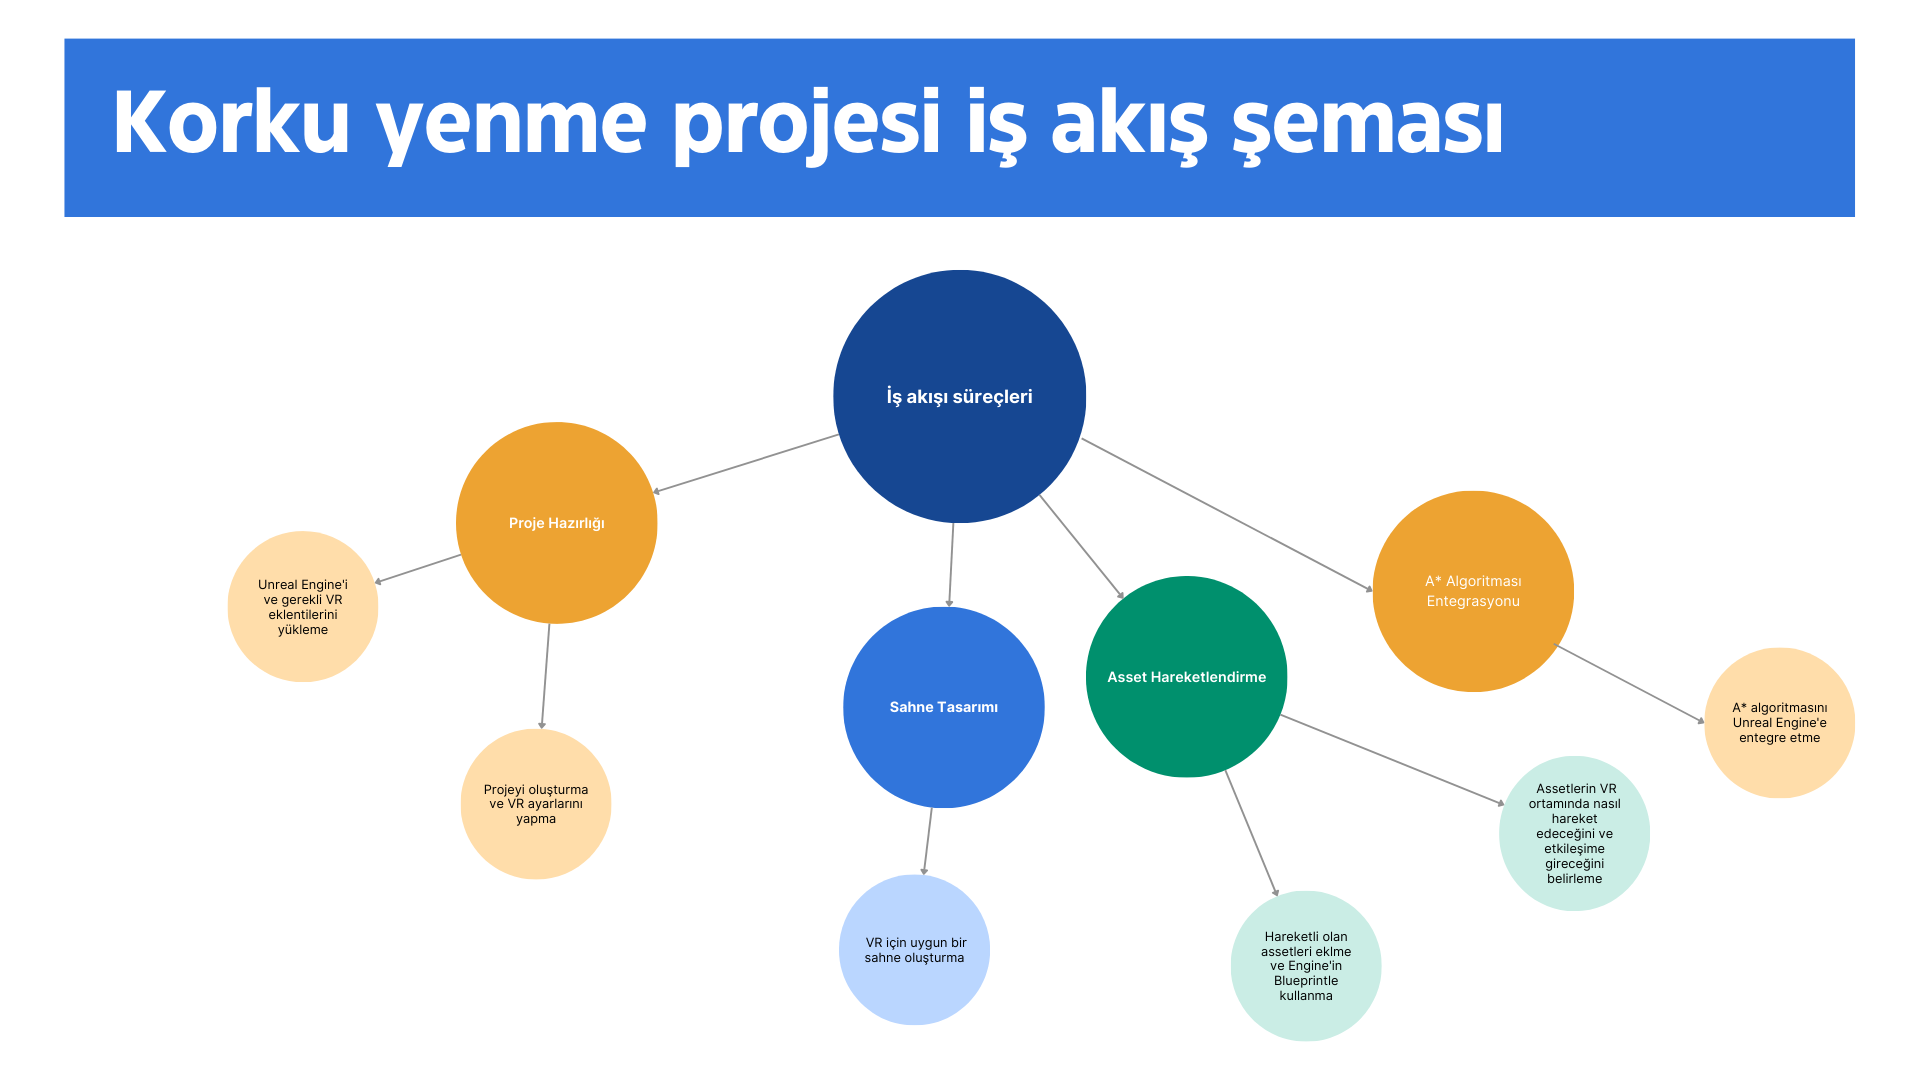
\includegraphics[width=0.9\textwidth ,height= 90mm ]{images/isakisi.png}\newline
		Projenin akış şeması yukarıdaki gibidir.\newline
	\end{figure}
	\begin{figure}[!htbp]
		\centering
		\caption{Gantt Chart}
		\centering
		%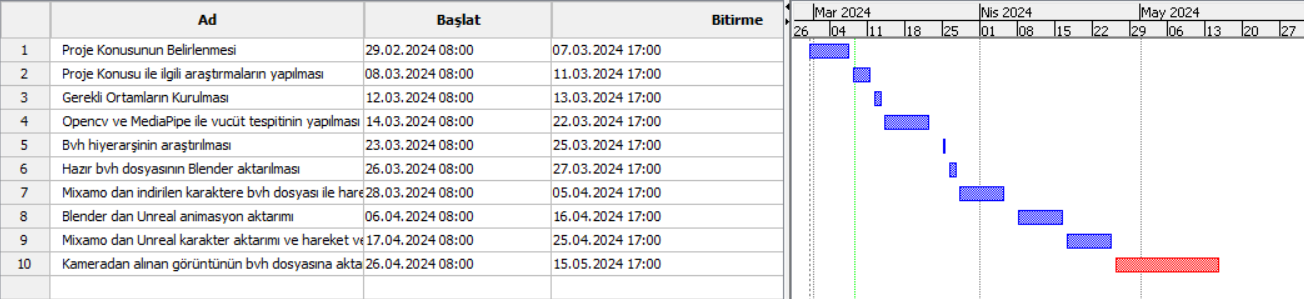
\includegraphics[angle=90, width=\textwidth]{x.png}
		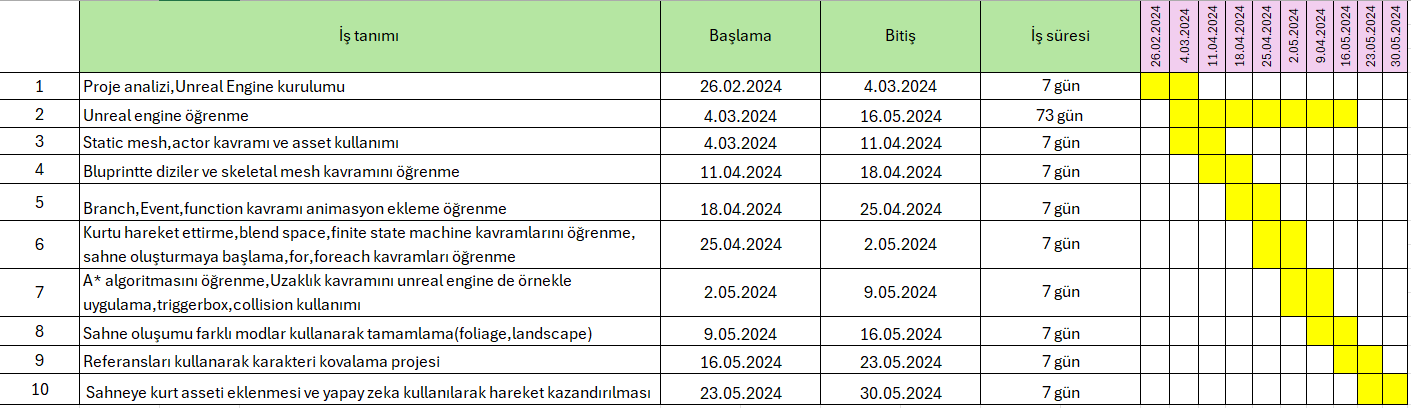
\includegraphics[height= 5 cm]{gantt.png}\newline
		\label{gantt}		
	\end{figure}  
		\section{Ayarlar \newline} 
		
	\begin{enumerate}
		\item Optimizasyon sağlama\newline
		project setting kısmından rendering kısmını seçtik.\newline
		Rendering: Oyunun görsel oluşturma ayarlarını içerir.\newline
		shadow kısmı: oyun içindeki gölgelerin nasıl görüneceğini kontrol eden aydınlatma ve gölgelendirme ayarlarıdır.\newline
		shadow kısmında ekran kartına binen yükü azaltmak için virtual shadow maps yerine shadow maps seçilmeli.\newline
		Shadow Maps (Gölge Haritaları): Klasik yöntem, hızlı ve verimlidir, basit sahneler için idealdir. Aliasing ve gölge akması gibi sorunlar yaşayabilir.\newline
		Virtual Shadow Maps (Sanal Gölge Haritaları): Daha yeni yöntem, daha yüksek kaliteli gölgeler, daha fazla ışık kaynağı ve karmaşık sahneler için uygundur. Daha fazla işlem gücü gerektirir ve yeni bir teknoloji olması nedeniyle riskler taşır.\newline
		
		reflection: reflection method kısmında none yaptık varsayılanı lumen
		reflections (yansımalar), bir sahnede bulunan nesnelerin diğer nesnelerin yüzeylerinde nasıl yansıdığını simüle ederek gerçekçi bir ortam oluşturmaya yardımcı olur.\newline
		
		Unreal Engine'de global illumination (GI), bir sahnede ışığın nesnelerle ve yüzeylerle nasıl etkileşim kurduğunu simüle ederek gerçekçi ışıklandırma efektleri oluşturma işlemidir. Bu, doğrudan ışık kaynaklarından aydınlatılmayan alanları aydınlatan, yüzeylerden yansıyan dolaylı ışığı da içerir.\newline
		
		gı altında dynamic global ıllumination method da varsayılan lumen seçili bunu none yaptık\newline
		lumen:Unreal Engine 5'te sunulan yeni bir gerçek zamanlı GI çözümüdür. Işın izleme gibi gelişmiş tekniklerden yararlanarak, yüksek kaliteli ve dinamik GI elde eder. Lumen, önceki yöntemlere göre daha iyi performans sunar ve karmaşık sahnelerde bile kullanılabilir.\newline
		
		Sağdaki settings kısmından gölgeler ışıklandırma yansıma en düşük ayarı verdik.	\newline\newline\newline
	    \item Blank projesinde third person karakteri kullanma 
	    	\begin{figure}[!htbp]
	    	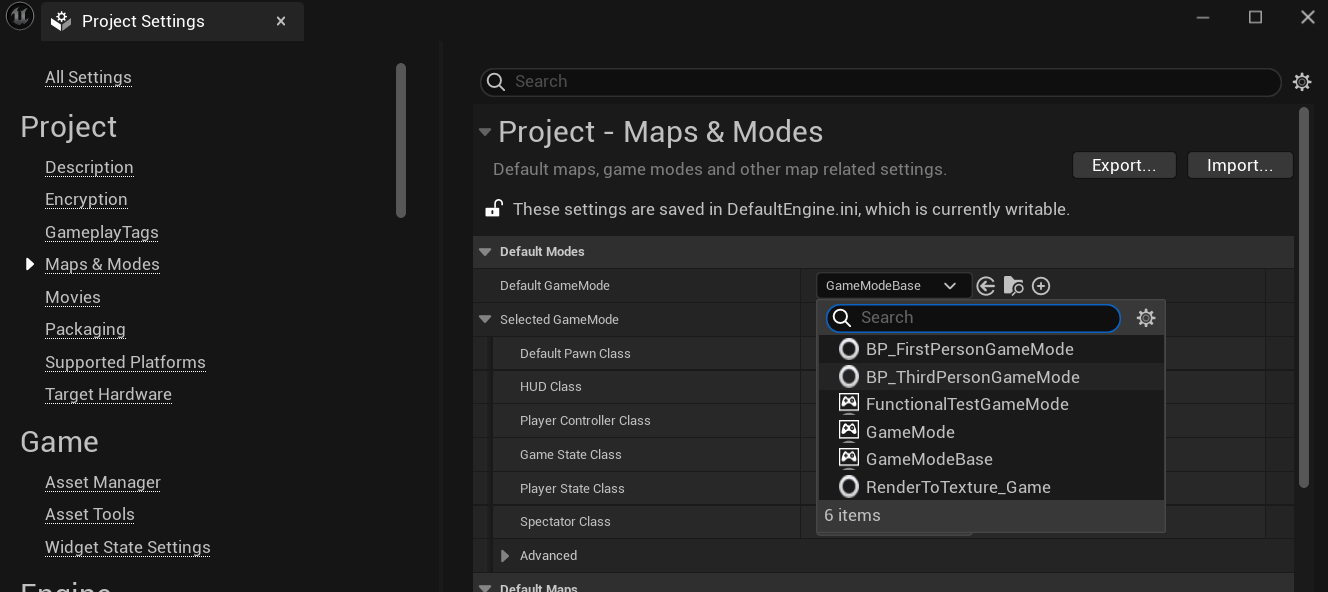
\includegraphics[width=0.7\textwidth,center]{images/blankmod.png}
	    	\caption{Blank projesine thirdperson ekleyip karakterle oyuna başlama}
	    	\label{fig:ornek}
	      \end{figure}
		
	\end{enumerate}
	\section{Hatalar \newline} 
	
	   
	\begin{enumerate}
		\item Asset eklendiğinde alınan hata
			\begin{center}
			\begin{figure}[!htbp]
				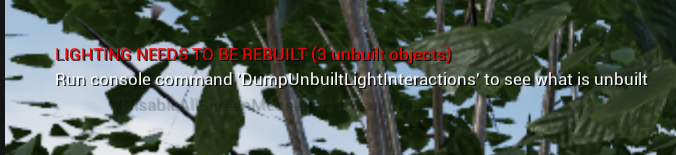
\includegraphics[width=0.7\textwidth,center]{images/ısıkhatasi.png}
				\caption{ışık hatası}
				\label{fig:ornek}
			\end{figure}
		\end{center}
		
		Build kısmından lighting quality kısmında normalde preview seçili biz production seçip  built lighting  only kısmını seçerek bu hatayı çözdük.\newline
		Lighting Quality:Oyunda kullanılacak aydınlatmanın kalitesini belirlemenizi sağlar.\newline
		Preview: Bu seçenek, aydınlatmanın hızlı ve düşük kaliteli bir önizlemesini verir. Bu, oyununuzun genel görünümünü hızlıca değerlendirmek için idealdir, ancak nihai ürün için kullanılmamalıdır.\newline
		Production: Bu seçenek, aydınlatmanın en yüksek kaliteli sürümünü oluşturur. Bu, gerçekçi ve ayrıntılı gölgeler ve aydınlatma efekti sağlar, ancak daha fazla işlem gücü ve zaman gerektirir.\newline
		Build Lighting Only: Bu seçenek, yalnızca aydınlatmayı oluşturur ve diğer oyun varlıklarını (örneğin dokular, sesler) oluşturmaz. Bu, aydınlatma değişikliklerini hızlı bir şekilde test etmek ve optimize etmek için yararlı olabilir.\vspace{0.5cm}
		\item Yapay zeka alanı (Nav mesh bounds volume) hatası
			
			\begin{figure}[!htbp]
				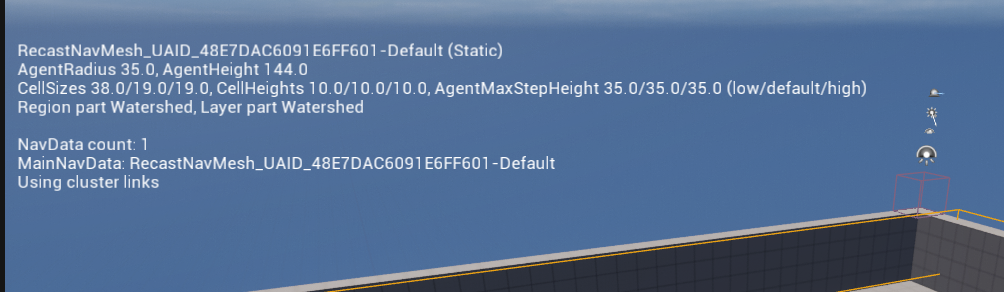
\includegraphics[width=0.7\textwidth,center]{images/aiyol.png}
				\caption{zemin hatası}
				\label{fig:ornek}
			\end{figure}

		Nav mesh bounds volume eklediğimiz zaman zemine temas etmeli.
		\item Referansın içi boş olma hatası
	
			\begin{figure}[!htbp]
				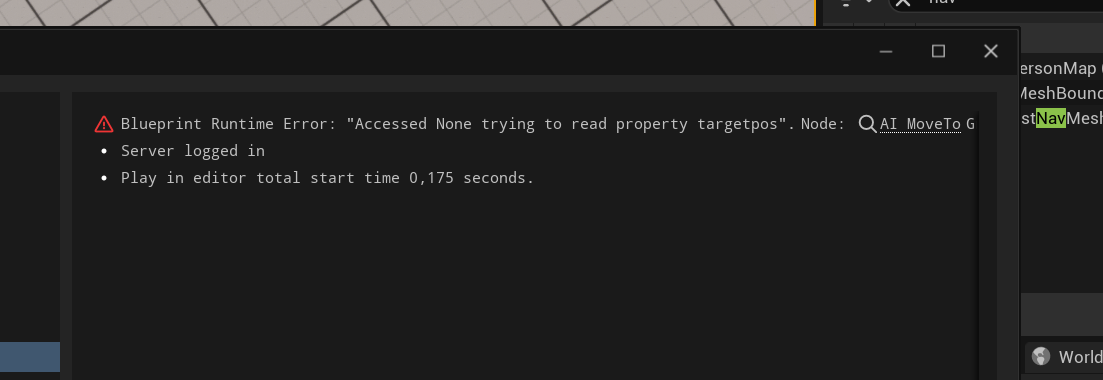
\includegraphics[width=0.7\textwidth,center]{images/refbos.png}
				\caption{Referans boş hatası}
				\label{fig:ornek}
			\end{figure}
		 Unreal Engine de referanslar 2 kısımda incelenir oyunda yer alan nesneler için (object reference,referans ver aktörü refererans verdiğimiz yerde details default  kısmından işaretle referans verdiğin aktörü Oyunda yer almayan nesneler için(class reference),referans verilecek kısımdan referans vereceğimiz aktör seçilir.Class ları kullanarak obejeleri oluştururuz. \cite{ref}.
		 	 	
		 	\begin{figure}[!htbp]
		 		\centering
		 		\begin{minipage}{0.45\textwidth}
		 			\centering
		 			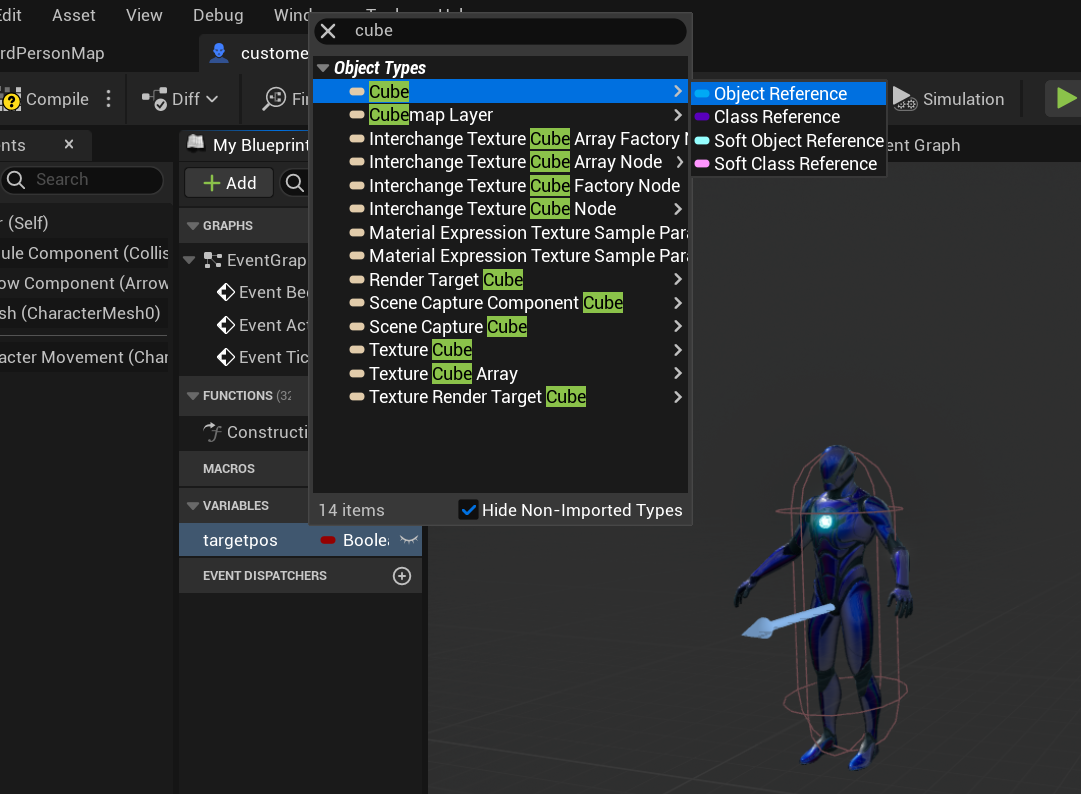
\includegraphics[width=7cm,height=7cm,keepaspectratio]{ref.png}
		 			\caption*{a)}
		 		\end{minipage}
		 		\hfill
		 		\begin{minipage}{0.45\textwidth}
		 			\centering
		 			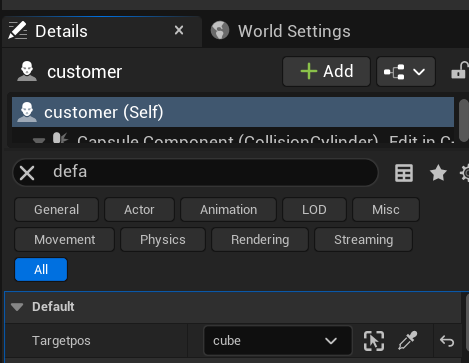
\includegraphics[width=7cm,height=7cm,keepaspectratio]{içidoldur.png}\newline
		 			\caption*{b)}
		 		\end{minipage}
		 		\caption{a) Obje referansı verme  b) Obje referansı doldurma}
		 	\end{figure}
		
		 \end{enumerate}
		
	 \section{Sonuç}
	Bu projede yapay zeka kullanılarak insanların köpek korkusunun önüne geçilmesi planlanmaktadır.Bu proje sayesinde insanların sokakta,köpek olan herhangi bir yerde korkusunu yenip aşırı tepki göstermemesi sonucuyla köpek saldırı vakaları azalabilir.
	\begin{figure}[!htbp]
		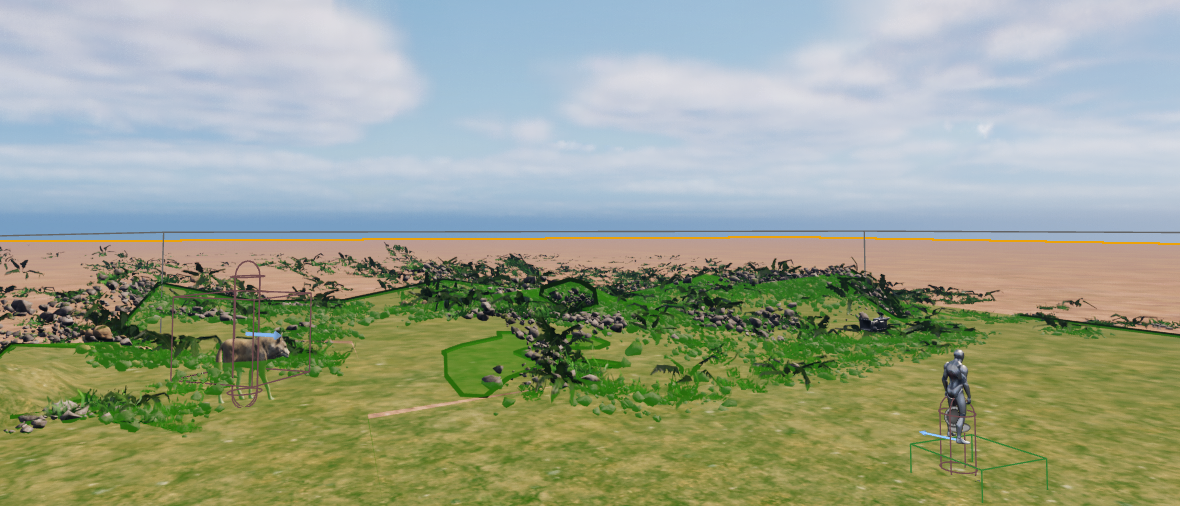
\includegraphics[width=0.7\textwidth,center]{images/sonsahne.png}
		\caption{Sahnenin son hali}
		\label{fig:ornek} 
	\end{figure}

	
	\bibliographystyle{ieeetr}
	\bibliography{kaynakca} 

\end{document}